% ============================================================
% CSE 8803 IUQ --- Final Presentation
% Bo Feng (bfeng66@gatech.edu)
% Beamer slide deck for the recorded video presentation
% ============================================================

\documentclass[10pt, aspectratio=169]{beamer}

\usetheme{metropolis}
\usepackage{amsmath, amssymb, bm}
\usepackage{booktabs}
\usepackage{microtype}
\usepackage{graphicx}
\usepackage{tikz}
\usepackage{hyperref}

\title{LLM-Informed Bayesian Priors}
\subtitle{Reducing Experimental Cost in Behavioral Economics}
\author{Bo Feng}
\institute{CSE 8803 IUQ \quad Spring 2026 \quad Georgia Tech}
\date{April 27, 2026}

\setbeamertemplate{footline}[frame number]
\setbeamertemplate{navigation symbols}{}

\begin{document}

% ============================================================
\maketitle

% ============================================================
\begin{frame}{The cost problem}
\begin{itemize}
  \item A behavioral economics study costs \textbf{\$10--\$50 per participant}, plus IRB and lab time.
  \item A typical condition needs \textbf{80--200 subjects} to estimate one parameter precisely.
  \item An LLM, prompted with the same instructions, produces \textbf{500 simulated decisions in minutes}.
\end{itemize}
\vspace{1em}
\begin{block}{Question}
  How much real data does an LLM prior save, and when does it break calibration?
\end{block}
\note{Recruiting 200 subjects easily costs ten thousand dollars and weeks of IRB. Meanwhile a
contemporary LLM responds to the same prompt the experimenter would read aloud, in seconds,
for cents. The natural UQ question: can we treat the LLM as an informative Bayesian prior?
That's the project.}
\end{frame}

% ============================================================
\begin{frame}{Setup}
\begin{columns}[T]
\begin{column}{0.5\textwidth}
\textbf{Data}
\begin{itemize}\setlength{\itemsep}{2pt}
  \item 137 dictator-game decisions
  \item von Blanckenburg et al., 2023
  \item 69 giving, 68 taking
  \item Train / test: 96 / 41 (30\%)
\end{itemize}
\vspace{0.5em}
\textbf{Likelihood}
\begin{equation*}
  y_i \mid \alpha, \beta \sim \mathrm{Beta}(\alpha, \beta), \quad \mu = \tfrac{\alpha}{\alpha+\beta}
\end{equation*}
\end{column}
\begin{column}{0.5\textwidth}
\textbf{Quantity of interest}
\begin{equation*}
  \rho = \frac{n^*_{\text{LLM}}}{n^*_{\text{flat}}}
\end{equation*}
$n^*$ is the smallest sample size to bring $\mathrm{Var}(\mu \mid \mathbf{y})$ below a target.
\vspace{0.4em}

$\rho < 1 \;\Rightarrow\;$ LLM prior saves human data.
\end{column}
\end{columns}
\note{The data: 137 individual decisions on dictator games where someone splits ten euros with
a stranger. We use the Beta likelihood for the share. The headline number is rho:
fraction of human sample size needed to reach the same precision when we have an LLM prior.}
\end{frame}

% ============================================================
\begin{frame}{Two methods}
\begin{columns}[T]
\begin{column}{0.5\textwidth}
\textbf{Baseline}: flat prior + MH-MCMC (log-space)
\begin{itemize}\setlength{\itemsep}{2pt}
  \item $p(\alpha,\beta) \propto 1$ on $(0, 100)^2$
  \item 15k samples, 3k burn-in
  \item Acceptance 0.22--0.58 \checkmark
\end{itemize}
\end{column}
\begin{column}{0.5\textwidth}
\textbf{Frontier}: LLM power prior + SVGD
\begin{itemize}\setlength{\itemsep}{2pt}
  \item $M=500$ pseudo-obs from GPT-4o
  \item $p_{\text{LLM}} \propto \prod_j \mathrm{Beta}(\tilde y_j; \alpha, \beta)^{w/M}$
  \item $w = 20$ effective weight
  \item SVGD: 100 particles, RBF kernel, Adam
\end{itemize}
\end{column}
\end{columns}
\vspace{1em}
\small
\begin{equation*}
  \bm{\eta}^{(k)}_{t+1} = \bm{\eta}^{(k)}_t + \tfrac{\epsilon}{K}\sum_{\ell=1}^K
  \!\left[\kappa(\bm{\eta}^{(\ell)}_t, \bm{\eta}^{(k)}_t)\,\nabla\!\log p(\bm{\eta}^{(\ell)}_t \mid \mathbf{y})
  + \nabla_{\bm{\eta}^{(\ell)}_t}\kappa(\bm{\eta}^{(\ell)}_t, \bm{\eta}^{(k)}_t)\right]
\end{equation*}
\note{The baseline is Metropolis-Hastings in log-space, which gives me positivity for free
with one Jacobian correction. The LLM power prior is a single-knob construction from
Ibrahim and Chen 2000: each pseudo-observation contributes weight w over M to the
log-likelihood. SVGD follows Liu and Wang 2016: an interacting particle system whose
update is the kernelised score.}
\end{frame}

% ============================================================
\begin{frame}{Main result: giving game}
\begin{columns}[T]
\begin{column}{0.6\textwidth}
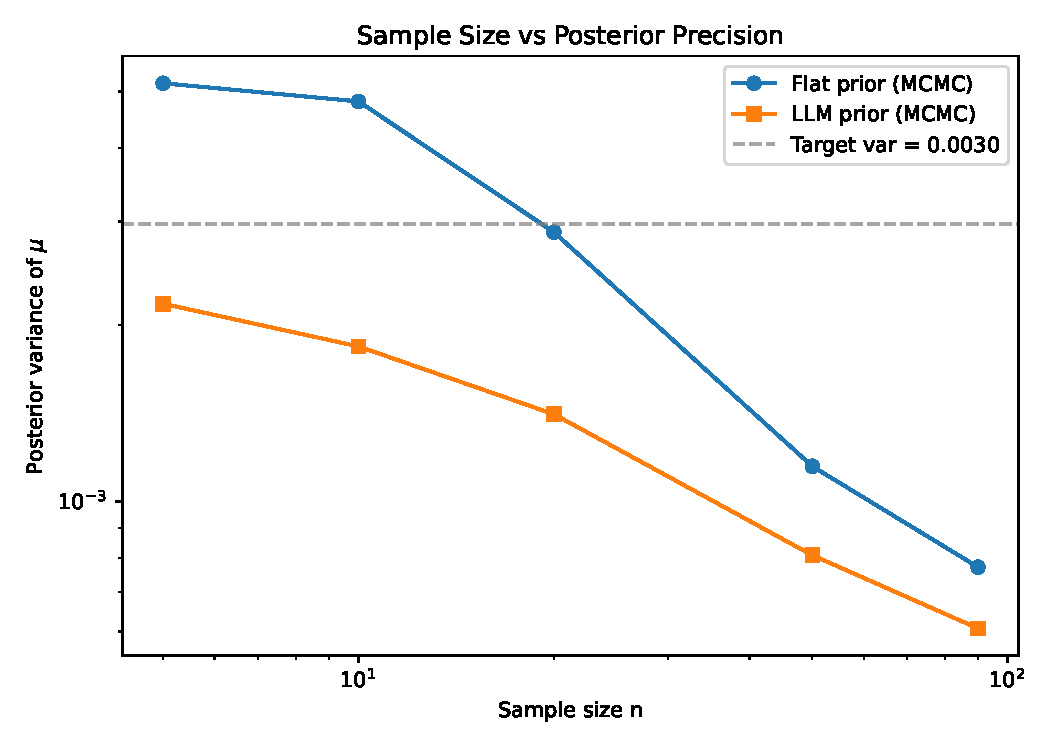
\includegraphics[width=\linewidth]{../../figures/nstar_curve.pdf}
\end{column}
\begin{column}{0.4\textwidth}
\small
\begin{tabular}{rl}
\toprule
$n$ & Var ratio \\
\midrule
5  & 2.38$\times$ \\
10 & 2.62$\times$ \\
20 & 2.04$\times$ \\
50 & 1.42$\times$ \\
90 & 1.27$\times$ \\
\bottomrule
\end{tabular}

\vspace{1em}
$n^*_{\text{flat}} = 19.2$ \\
$n^*_{\text{LLM}} = 5.0$

\vspace{0.3em}
\textbf{$\rho = 0.26$}

74\% smaller human sample to reach the same precision.
\end{column}
\end{columns}
\note{Headline result on the giving game. The LLM prior cuts the human sample to roughly
one-quarter. Most of the gain is at small n, which makes sense: the prior contributes
twenty effective pseudo-observations, so when you only have five humans, twenty-five over
five equals five-x improvement is the analytic ceiling.}
\end{frame}

% ============================================================
\begin{frame}{Cross-game replication: taking game}
\begin{columns}[T]
\begin{column}{0.6\textwidth}
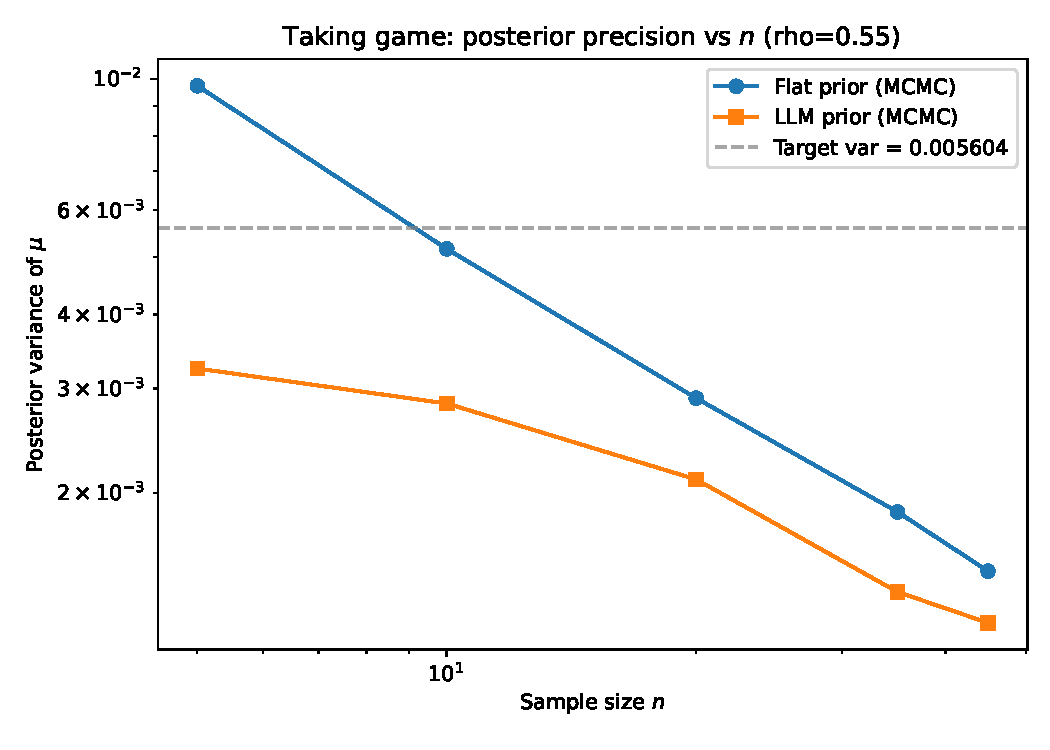
\includegraphics[width=\linewidth]{../../figures/nstar_curve_taking.pdf}
\end{column}
\begin{column}{0.4\textwidth}
\small
\begin{tabular}{rl}
\toprule
$n$ & Var ratio \\
\midrule
5  & 3.00$\times$ \\
10 & 1.82$\times$ \\
20 & 1.37$\times$ \\
35 & 1.36$\times$ \\
45 & 1.22$\times$ \\
\bottomrule
\end{tabular}

\vspace{1em}
$\rho_{\text{taking}} = 0.55$

vs.\ $\rho_{\text{giving}} = 0.26$

\vspace{0.3em}
\textbf{The LLM prior generalises -- partially.}
\end{column}
\end{columns}
\note{Phillip's strongest suggestion: do this on the taking game. Result: rho equals
zero point five five, twice as high. Why? GPT-4o under the taking prompt has counterpart
kept share of zero point five two, but humans in the taking game keep only zero point
three four. Humans take more aggressively than the LLM. The LLM generalises the
protocol but not the framing-induced behavioural shift.}
\end{frame}

% ============================================================
\begin{frame}{Failure mode: dense misspecification curve}
\begin{columns}[T]
\begin{column}{0.6\textwidth}
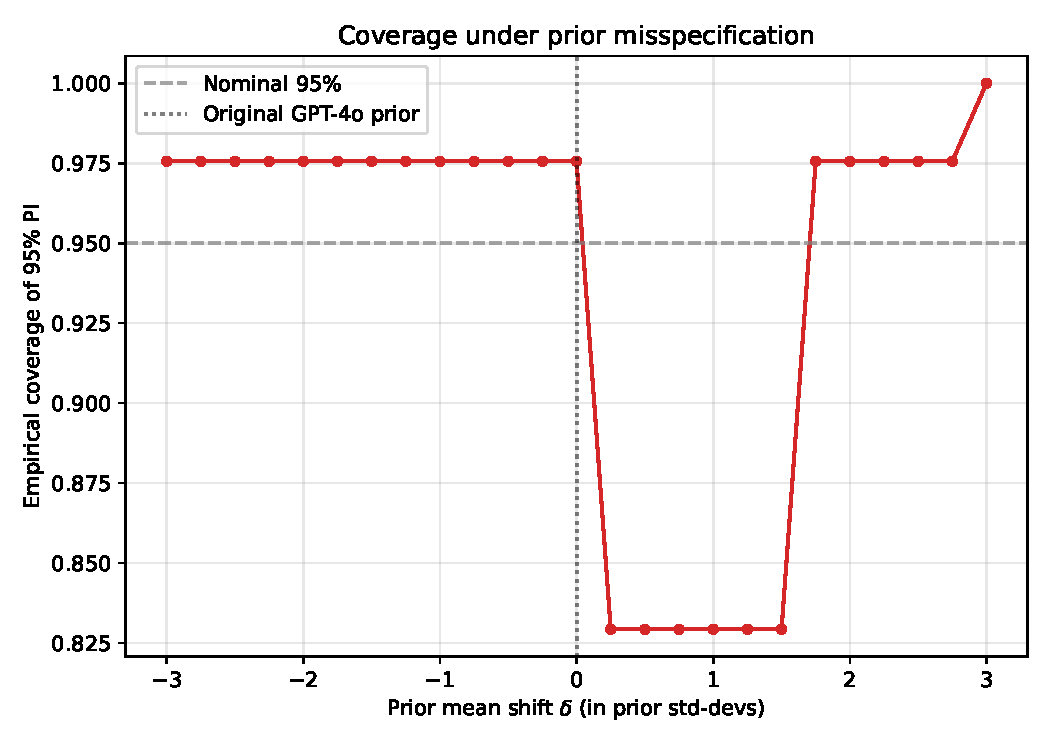
\includegraphics[width=\linewidth]{../../figures/failure_mode_dense.pdf}
\end{column}
\begin{column}{0.4\textwidth}
\small
\begin{itemize}\setlength{\itemsep}{4pt}
  \item Shift LLM prior by $\delta$ prior std-deviations
  \item Coverage of nominal-95\% PI on held-out
\end{itemize}
\textbf{Asymmetric failure}:
\begin{itemize}\setlength{\itemsep}{2pt}
  \item $\delta \le 0$: stays calibrated
  \item $\delta \in [+0.25, +1.5]$: coverage drops to 0.83
  \item $\delta \ge +1.75$: data wins
\end{itemize}
\vspace{0.5em}
\textbf{Moderate misspecification is the dangerous regime}.
\end{column}
\end{columns}
\note{This is the failure mode I would worry about in deployment: not a totally wrong
prior, but a prior that is about one standard deviation off in the bad direction. The
data won't override it. The check-in had this as a five-point table; here it is a
continuous curve with a clear plateau.}
\end{frame}

% ============================================================
\begin{frame}{Compute--accuracy: MCMC vs SVGD}
\centering
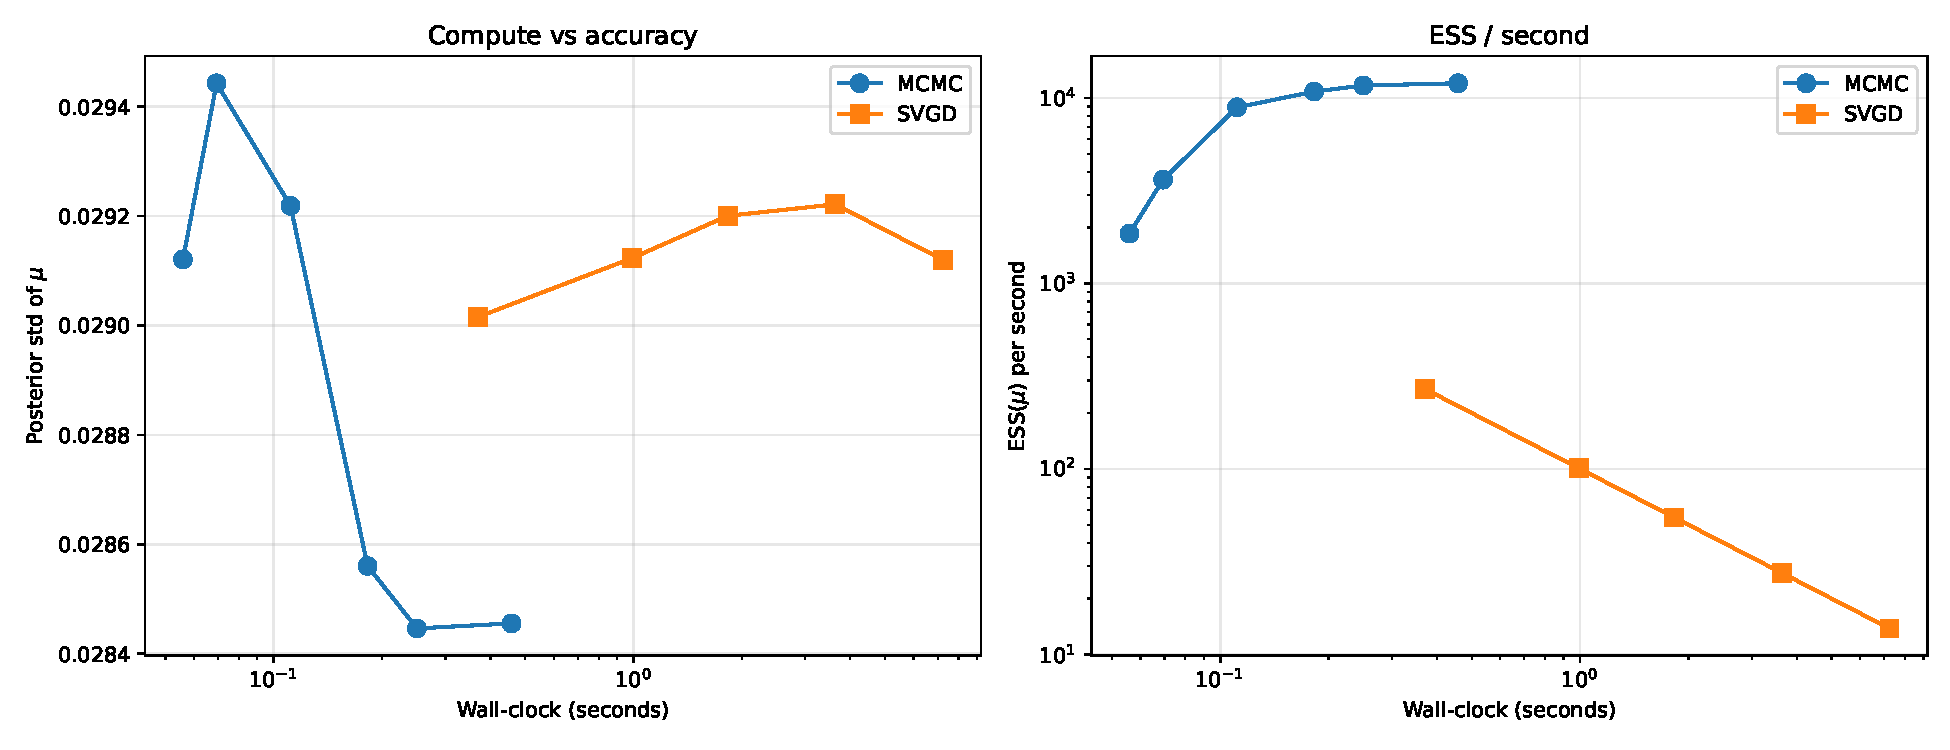
\includegraphics[height=0.55\textheight]{../../figures/pareto.pdf}

\vspace{0.5em}
\small
\begin{columns}[T]
\begin{column}{0.5\textwidth}
\textbf{MCMC at $d=2$}: ESS/sec $\approx 1.2 \times 10^4$\\
\textbf{SVGD at $d=2$}: ESS/sec $\approx 14$--$270$
\end{column}
\begin{column}{0.5\textwidth}
For this 2-parameter Beta posterior, MCMC dominates SVGD by $\sim$100$\times$.

SVGD's value is in higher-d posteriors with multi-modality, not here.
\end{column}
\end{columns}
\note{Honest reporting: at d equals two with a unimodal Beta posterior, MH-MCMC eats
SVGD's lunch. Two orders of magnitude in ESS per second. Why include SVGD then? Because
in the hierarchical extension I sketch in the discussion, MCMC mixing degrades and
SVGD's particle update doesn't.}
\end{frame}

% ============================================================
\begin{frame}{Leakage check: gpt-3.5-turbo (Sep 2021 cutoff)}
\centering
\small
\begin{tabular}{lcccc}
\toprule
Model & Cutoff & Prior mean & $\rho$ & Coverage ($n=50$) \\
\midrule
gpt-4o        & 2023-10 & 0.299 & \textbf{0.261} & \textbf{0.976} \\
gpt-3.5-turbo & 2021-09 (pre-Horton) & 0.548 & \textbf{0.261} & \textbf{0.829} \\
\bottomrule
\end{tabular}

\vspace{1em}
\begin{itemize}\setlength{\itemsep}{4pt}
  \item \textbf{Sample-size reduction is identical}: $\rho_{\text{gpt-3.5}} = \rho_{\text{gpt-4o}}$ to 3 sig figs $\Rightarrow$ \emph{not a leakage artefact}.
  \item \textbf{Calibration is not}: gpt-3.5 prior mean is $0.55$, far above the human mean of $0.36$.
  \item Power prior: variance benefit driven by $w$; calibration driven by prior \emph{location}.
\end{itemize}
\note{The cleanest single ablation in the project. gpt-3.5 with a September 2021 cutoff
predates the Horton paper. Same rho. Different calibration. So whatever the LLM prior
does for sample size, it doesn't seem to be a memorisation trick. But the calibration
gap shows gpt-4o still has some advantage in prior location that I cannot fully separate
from training-data overlap.}
\end{frame}

% ============================================================
\begin{frame}{Limitations}
\begin{columns}[T]
\begin{column}{0.5\textwidth}
\textbf{Identified}
\begin{itemize}\setlength{\itemsep}{2pt}
  \item LLM under-takes vs humans in taking-game framing
  \item Asymmetric coverage trough at $\delta \approx +1$
  \item $w=20$ is a knob, not optimised
  \item 2-d posterior is too small for SVGD to win
  \item German university student sample $\ne$ LLM persona
\end{itemize}
\end{column}
\begin{column}{0.5\textwidth}
\textbf{What's next}
\begin{itemize}\setlength{\itemsep}{2pt}
  \item Hierarchical $(\alpha_g, \beta_g, \alpha_t, \beta_t, \tau)$ joint model -- SVGD becomes essential at $d \ge 4$
  \item Predictive log-likelihood to optimise $w$
  \item Multiple LLM corpora to disentangle leakage from prior-location quality
  \item Out-of-domain games where LLM training is sparse
\end{itemize}
\end{column}
\end{columns}
\note{The honest list. The biggest one: I never actually tested SVGD in the regime where
it would dominate MCMC, because I only ever inferred two parameters. The natural
extension is a hierarchical model across both game variants. That gets you to five
parameters with correlations, and is exactly the d-regime where SVGD's particle update
would amortise.}
\end{frame}

% ============================================================
\begin{frame}{Takeaways}
\begin{itemize}\setlength{\itemsep}{6pt}
  \item $\rho \approx 0.26$ on the giving game: GPT-4o saves $\sim$74\% of the human sample.
  \item $\rho \approx 0.55$ on the taking game: LLM prior generalises across protocols, not framings.
  \item Calibration: nominal at unshifted prior; trough at moderate upward shift, not at extreme shifts.
  \item Leakage: not the source of the sample-size benefit, but plausibly part of why gpt-4o has a better-located prior than gpt-3.5.
  \item SVGD vs MCMC at $d=2$: MCMC wins by 100$\times$ in ESS/sec; SVGD's value awaits the higher-d hierarchical extension.
\end{itemize}
\vspace{0.6em}
\centering\small
\href{https://github.gatech.edu/bfeng66/cse8803-iuq-project}{github.gatech.edu/bfeng66/cse8803-iuq-project}
\note{To wrap up: rho around zero point two six on the headline experiment, zero point
five five on the cross-game replication, calibration is good outside of moderately
misspecified upward shifts, the leakage ablation cleanly disentangles variance shrinkage
from prior-location quality, and SVGD waits for the higher-dimensional sequel. Thanks;
I'm happy to take questions.}
\end{frame}

% ============================================================
\begin{frame}[fragile]{Backup: reproduce in $<$1 hour}
\begin{verbatim}
conda activate base   # numpy / scipy / matplotlib / openai
python scripts/run_experiment.py            # rho ~ 0.26 on giving game
python scripts/run_experiment_taking.py     # rho ~ 0.55 on taking game
python scripts/run_experiment_gpt35.py      # gpt-3.5 leakage ablation
python scripts/run_failure_mode_dense.py    # 25-point misspecification grid
python scripts/run_compute_pareto.py        # MCMC vs SVGD Pareto
\end{verbatim}
\begin{itemize}\setlength{\itemsep}{2pt}
  \item All seeds fixed at 42
  \item Elicited LLM pseudo-data committed to \texttt{data/llm\_prior\_samples*.npy}
  \item API key in \texttt{.env} required only for re-elicitation
\end{itemize}
\end{frame}

\end{document}
